\documentclass{article}
\addtolength{\oddsidemargin}{-1.cm}
\addtolength{\textwidth}{2cm}
\addtolength{\topmargin}{-2cm}
\addtolength{\textheight}{3.5cm}
\newcommand{\HRule}{\rule{\linewidth}{0.5mm}}
\makeindex

\usepackage{longtable}
\usepackage[pdftex]{graphicx}
\usepackage{makeidx}
\usepackage{hyperref}



\usepackage{changepage,lipsum,titlesec}% http://ctan.org/pkg/{changepage,lipsum,titlesec}
\titleformat{\section}[block]{\bfseries}{\thesection.}{1em}{}
\titleformat{\subsection}[block]{}{\thesubsection}{1em}{}
\titleformat{\subsubsection}[block]{}{\thesubsubsection}{1em}{}
\titlespacing*{\subsection} {2em}{3.25ex plus 1ex minus .2ex}{1.5ex plus .2ex}
\titlespacing*{\subsubsection} {3em}{3.25ex plus 1ex minus .2ex}{1.5ex plus .2ex}

\setlength\parindent{74pt}
 
\hypersetup{
	colorlinks=true,
	linkcolor=black,
	filecolor=magenta,      
	urlcolor=cyan,
}


% define the title
\author{Team now.next}
\title{ Software Requirements Specification}
\begin{document}
	\setlength{\parskip}{6pt}
	
	% generates the title
	\begin{titlepage}
		
		\begin{center}
			% Upper part of the page       
		
			\textsc{\LARGE Department of Computer Science}\\[1.5cm]
			\textsc{\Large COS 301 - Software Engineering}\\[0.5cm]
			% Title
			\HRule \\[0.4cm]
			%%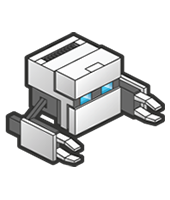
\includegraphics[width=0.05\textwidth]{./logo.png}\\[0.4cm] 
			{ \huge \bfseries Software Requirements Specification}\\[0.4cm]
			\HRule \\[0.4cm]
			% Author and supervisor
			\begin{minipage}{0.4\textwidth}
				\begin{flushleft} \large
					\emph{Authors:}
				\end{flushleft}
			\end{minipage}
			\begin{minipage}{0.4\textwidth}
				\begin{flushright} \large
					\emph{Student number:}
				\end{flushright}
			\end{minipage}
			
			\begin{minipage}{0.4\textwidth}
				\begin{flushleft} \large
					Vuyani {Shabangu}
				\end{flushleft}
			\end{minipage}
			\begin{minipage}{0.4\textwidth}
				\begin{flushright} \large
					\emph{}
					11171139
				\end{flushright}
			\end{minipage}
			
			\begin{minipage}{0.4\textwidth}
				\begin{flushleft} \large
					Sibusiso {Masemola}
				\end{flushleft}
			\end{minipage}
			\begin{minipage}{0.4\textwidth}
				\begin{flushright} \large
					\emph{}
					12270467
				\end{flushright}
			\end{minipage}
			
			\begin{minipage}{0.4\textwidth}
				\begin{flushleft} \large
					Sello {Thosago}
				\end{flushleft}
			\end{minipage}
			\begin{minipage}{0.4\textwidth}
				\begin{flushright} \large
					\emph{}
					13062060
				\end{flushright}
			\end{minipage}
			
			\begin{minipage}{0.4\textwidth}
				\begin{flushleft} \large
					Banele {Nxumalo}
				\end{flushleft}
			\end{minipage}
			\begin{minipage}{0.4\textwidth}
				\begin{flushright} \large
					\emph{}
					12201911
				\end{flushright}
			\end{minipage}
			
			\begin{minipage}{0.4\textwidth}
				\begin{flushleft} \large
					Aiden {Malan}
				\end{flushleft}
			\end{minipage}
			\begin{minipage}{0.4\textwidth}
				\begin{flushright} \large
					\emph{}
					12265731
				\end{flushright}
			\end{minipage}
			
			
			\vfill
			
		\end{center}
	\end{titlepage}
	\footnotesize
	%\input{declaration_of_originality.tex}
	\normalsize
	
	
	\pagenumbering{roman}
	\tableofcontents
	\newpage
	\pagenumbering{arabic}
	
	\newpage %Aiden malan
	\section{Introduction} 
	\begin{itemize} 
		\item The vision.
		\item The background.
	\end{itemize}
	
	\section{Vision}%%aiden
	
	
	\section{Background} %%aiden

	\newpage
	
	\section{Architecture Requirements}%Header
		\subsection{Architectural Scope}%%Aiden
		%Here just talk about overview of the architectural requirements. Just broadly what the quality of the product must be.
		
			\setlength{\leftskip}{45px}
				\lipsum[2]

		\subsection{Quality Requirements}%%Vuyani
			The following is a list of quality requirements that have been established by the product owner that the system must posses.
			\subsubsection{Stability}
				\setlength{\leftskip}{61px}
			 	
		\subsection{Integration and Access Channel Requirements}%%Sello
		%Here just speak about what the system is expected to integrate with. Write about how it is suppose to be accessable to 			%web for users and operators.  It must also be able to interact with different types of drones.
		\subsection{Architectural Constraints }%%Banele
		%Talk about the constraints that we might have in producing the architecture that they have asked for.
	\section{Architectural patterns}%%Sibusiso MVC, layered
	%Write that we are using a hybrid of MVC and Layered pattern (MVC to support the web part of the system, and layered to 		%support the intergability required by the part of the system that talks to the drones)
	\section{Architectural Tactics}%%Banele
	%use the same tactics that we spoke about in the presentation, discuss them more in detail
	\section{Access and Integration channels}%%Sello
	%This time, you are writing about the how we will meet the intergration requirements that you wrote about earlier. Write about how 	%we will use a HTTPS REST API to interact with the web portal. Talk about our layered approach to interacting with the drones; 	%our system->drone interfacing object -> adrupilot -> pixhawk -> drone.
	\section{Technologies}%%Sibusiso
	%List and describe all the technologies we will be using, including why we are using them. Make sure for each one you mention 	%how it solves an architectural requirement.
	%MEAN Stack (Mongo, ExpressJS, AngualrJS, NodeJS), Mongoose (for ORM), Heroku Server, Travis for CI... and others
	
	
	
	
	
	
\end{document}
